%%%%%%%%%%%%%%%%%%%%%%%%%%%%%%%%%%%%%%%%%%%%%%%%%%%%%%%%%%%%%%%%%%%%%%%%
\chapter{Implementation}
%%%%%%%%%%%%%%%%%%%%%%%%%%%%%%%%%%%%%%%%%%%%%%%%%%%%%%%%%%%%%%%%%%%%%%%%
We implement our design using Deep Graph Library (DGL) \cite{DGL_2019}, a GNN training framework; PyTorch \cite{PyTorch_2019} a tensor operation library; and a mix of Python and C++.
Our current implementation consists of roughly 5,000 SLOC of Python and 1,000 SLOC of C++, and is publicly available at \url{https://github.com/henryliu5/thesis}.
\begin{figure}[h!]
    \centering
    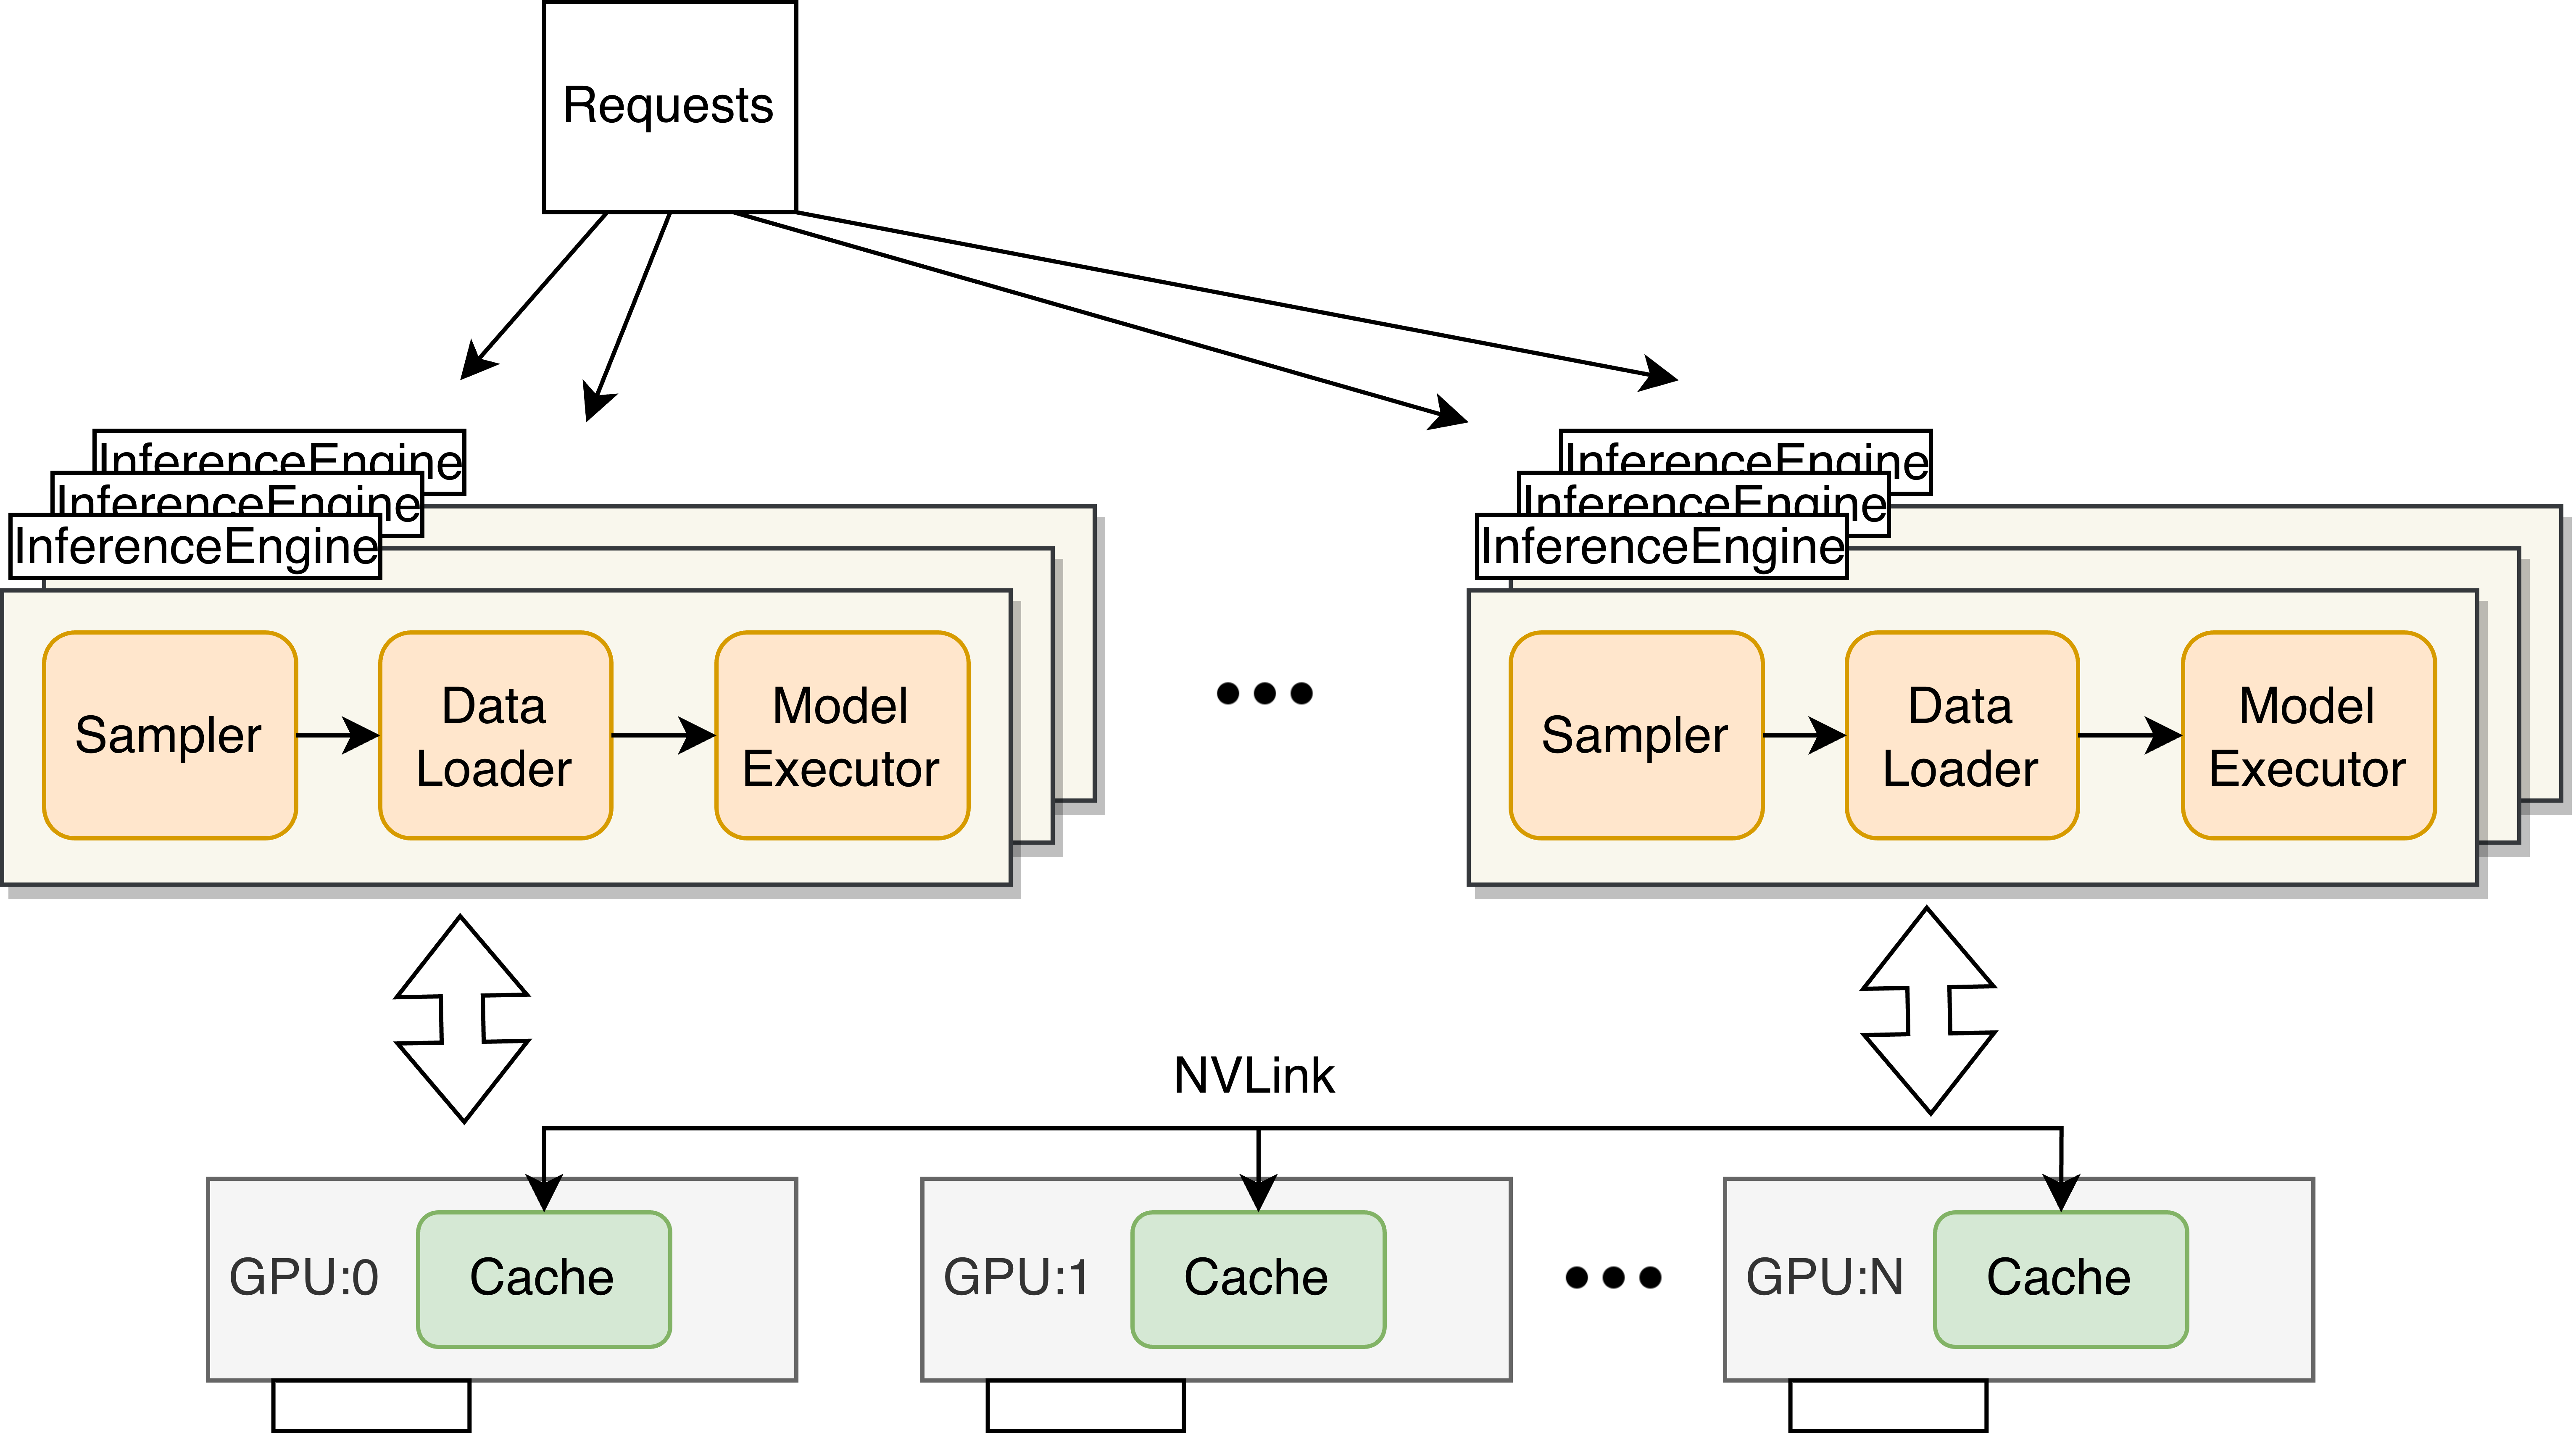
\includegraphics[width=\textwidth]{diagrams/group_meeting_gnn-System Diagram.png}
    
    \caption{System diagram}
    \label{Our system diagram}
\end{figure} 
\\ \\
\noindent \textbf{InferenceEngine Abstraction} \quad Due to Python's global interpreter lock, we leverage multiprocessing as the primary vehicle for inter-request concurrency. Our InferenceEngine abstraction represents a single process, which performs all operations for a single inference request - sampling, data loading, and model execution - sequentially. By binding InferenceEngines to a single GPU and containing these steps within a single process, we avoid any overheads due to IPC serialization. Multiple InferenceEngines can be created per GPU, which share GPU and host memory for resources such as model weights and graph features. All InferenceEngines share a request queue and response queue to receive inference requests and send back results. The InferenceEngine API supports any models or graph datasets that are built using DGL.
\\ \\ 
\noindent \textbf{Asynchronous Cache Update Thread Control} \quad Each InferenceEngine has a special C++ cache update thread linked using pybind11 \cite{pybind11} to perform cache update operations. Atomic integers required for masked cache updates are placed in shared memory using Boost \cite{BoostLibrary}. We also have one shared memory mutex per GPU to allow only one InferenceEngine's update thread to actively write at once. If the update thread fails to immediately acquire the lock, the update is skipped.
\\ \\
\noindent \textbf{GPU Sampling} \quad We use DGL's implementation of GPU sampling to perform the sampling stage. This requires graph structure (no features) to somehow be present in GPU memory. If graph structure can fit in a single GPU's memory, then the entire graph structure is copied to GPU memory during system initialization. If graph structure does not fit in GPU memory, we fall back to DGL's zero-copy functionality that allows GPUs to directly pull graph structure information from host memory when necessary \cite{PyTorch_Direct_2021}. 
\\ \\
\noindent \textbf{CUDA Multi-Process Serivce (MPS) \cite{CUDA_MPS}} \quad
To enable concurrent concurrent GPU kernel execution among InferenceEngines, we use NVIDIA CUDA MPS to provide a single CUDA context for all InferenceEngine processes. This is crucial for maximizing GPU utilization and avoiding unnecessary serialization of kernels, as many GPU kernels in our system do not fully occupy all SMs.

\section{Limitations}
Our system currently does not combine new inference requests into the existing graph or retrain the GNN to accommodate for new requests. 
Instead, we look only at GNN computation and investigate how to efficiently compute new embeddings. 
Integrating new nodes into the existing graph and dealing with challenges such as consistency are both orthogonal and out of scope of this work, but would be an interesting and natural extension.
